In authentication, when the user successfully logs in using their credentials, a JSON Web Token will be returned.
Since tokens are credentials, great care must be taken to prevent security issues.
In general, you should not keep tokens longer than required.
You also should not store sensitive session data in browser storage due to lack of security.
Whenever the user wants to access a protected route or resource, the user agent should send the JWT,
typically in the Authorization header using the Bearer schema.
The content of the header should look like the following:
\begin{spverbatim}

    Authorization: Bearer <token>

\end{spverbatim}
This can be, in certain cases, a stateless authorization mechanism.
The server's protected routes will check for a valid JWT in the Authorization header, and if it's present,
the user will be allowed to access protected resources.
If the JWT contains the necessary data, the need to query the database for certain operations may be reduced,
though this may not always be the case.
If the token is sent in the Authorization header, Cross-Origin Resource Sharing (CORS) won't be an issue
as it doesn't use cookies.
Generally, the workflow is as follows
% old
\begin{enumerate}
    \item The user has been successfully authenticated using their credentials.
    \item The server checks in database the roles and other claims of the user.
    \item The server generated token with specified roles and claims.
    \item User requests resource using received token passed to the request header.
    \item The server check user's claims and proceeds or declines request.
\end{enumerate}

The fifth point is the authorization.
As a result, token stored on the client and used when it is necessary to authorize the requests.
When a hacker tries to replace the data in the header or payload the token will become invalid,
therefore the signature will not match the original values.
So, the hacker hasn't any possibility to generate a new signature since that encryption secret key stored on the server.
Access token (JWT) is used for request authorization and for storing the additional information about user like identifier,
display name and others.

Refresh Token (GUID) issued by server based on successful authentication results and used for get new access/refresh
token pair.
Every token has its own lifetime.
For example, Access token's lifetime may be 5 minutes, and Refresh token's 7 days.

\subsection{Creating sessions}\label{subsec:creating-sessions}

\begin{enumerate}
    \item The user logs into the application by transferring the login, password and fingerprint of the browser,
    or some other unique device identifier if it is not a browser.
    \item The server verifies the authenticity of the login and password.
    \item If successful, creates and writes a session to the database, see table session in
    [REFERENCE\_DATABASE\_SCHEMA].
    \item The server generates Access token.
    \item The server sends to client access token and refresh token, UUID\@.
    \item Client saves the pair of access and refresh tokens.
\end{enumerate}

Before each request client preliminarily checks access token's lifetime and if it expired, client sends request for
updating access token.
For more confidence, we can update tokens a few seconds earlier.
That is, the case when the API receives an expired access token is practically excluded.
To use the authentication feature on more than one device, it is necessary to store all refresh tokens for each user.
The following diagram demonstrates discussed processes

\begin{figure}[H]
    \centering
    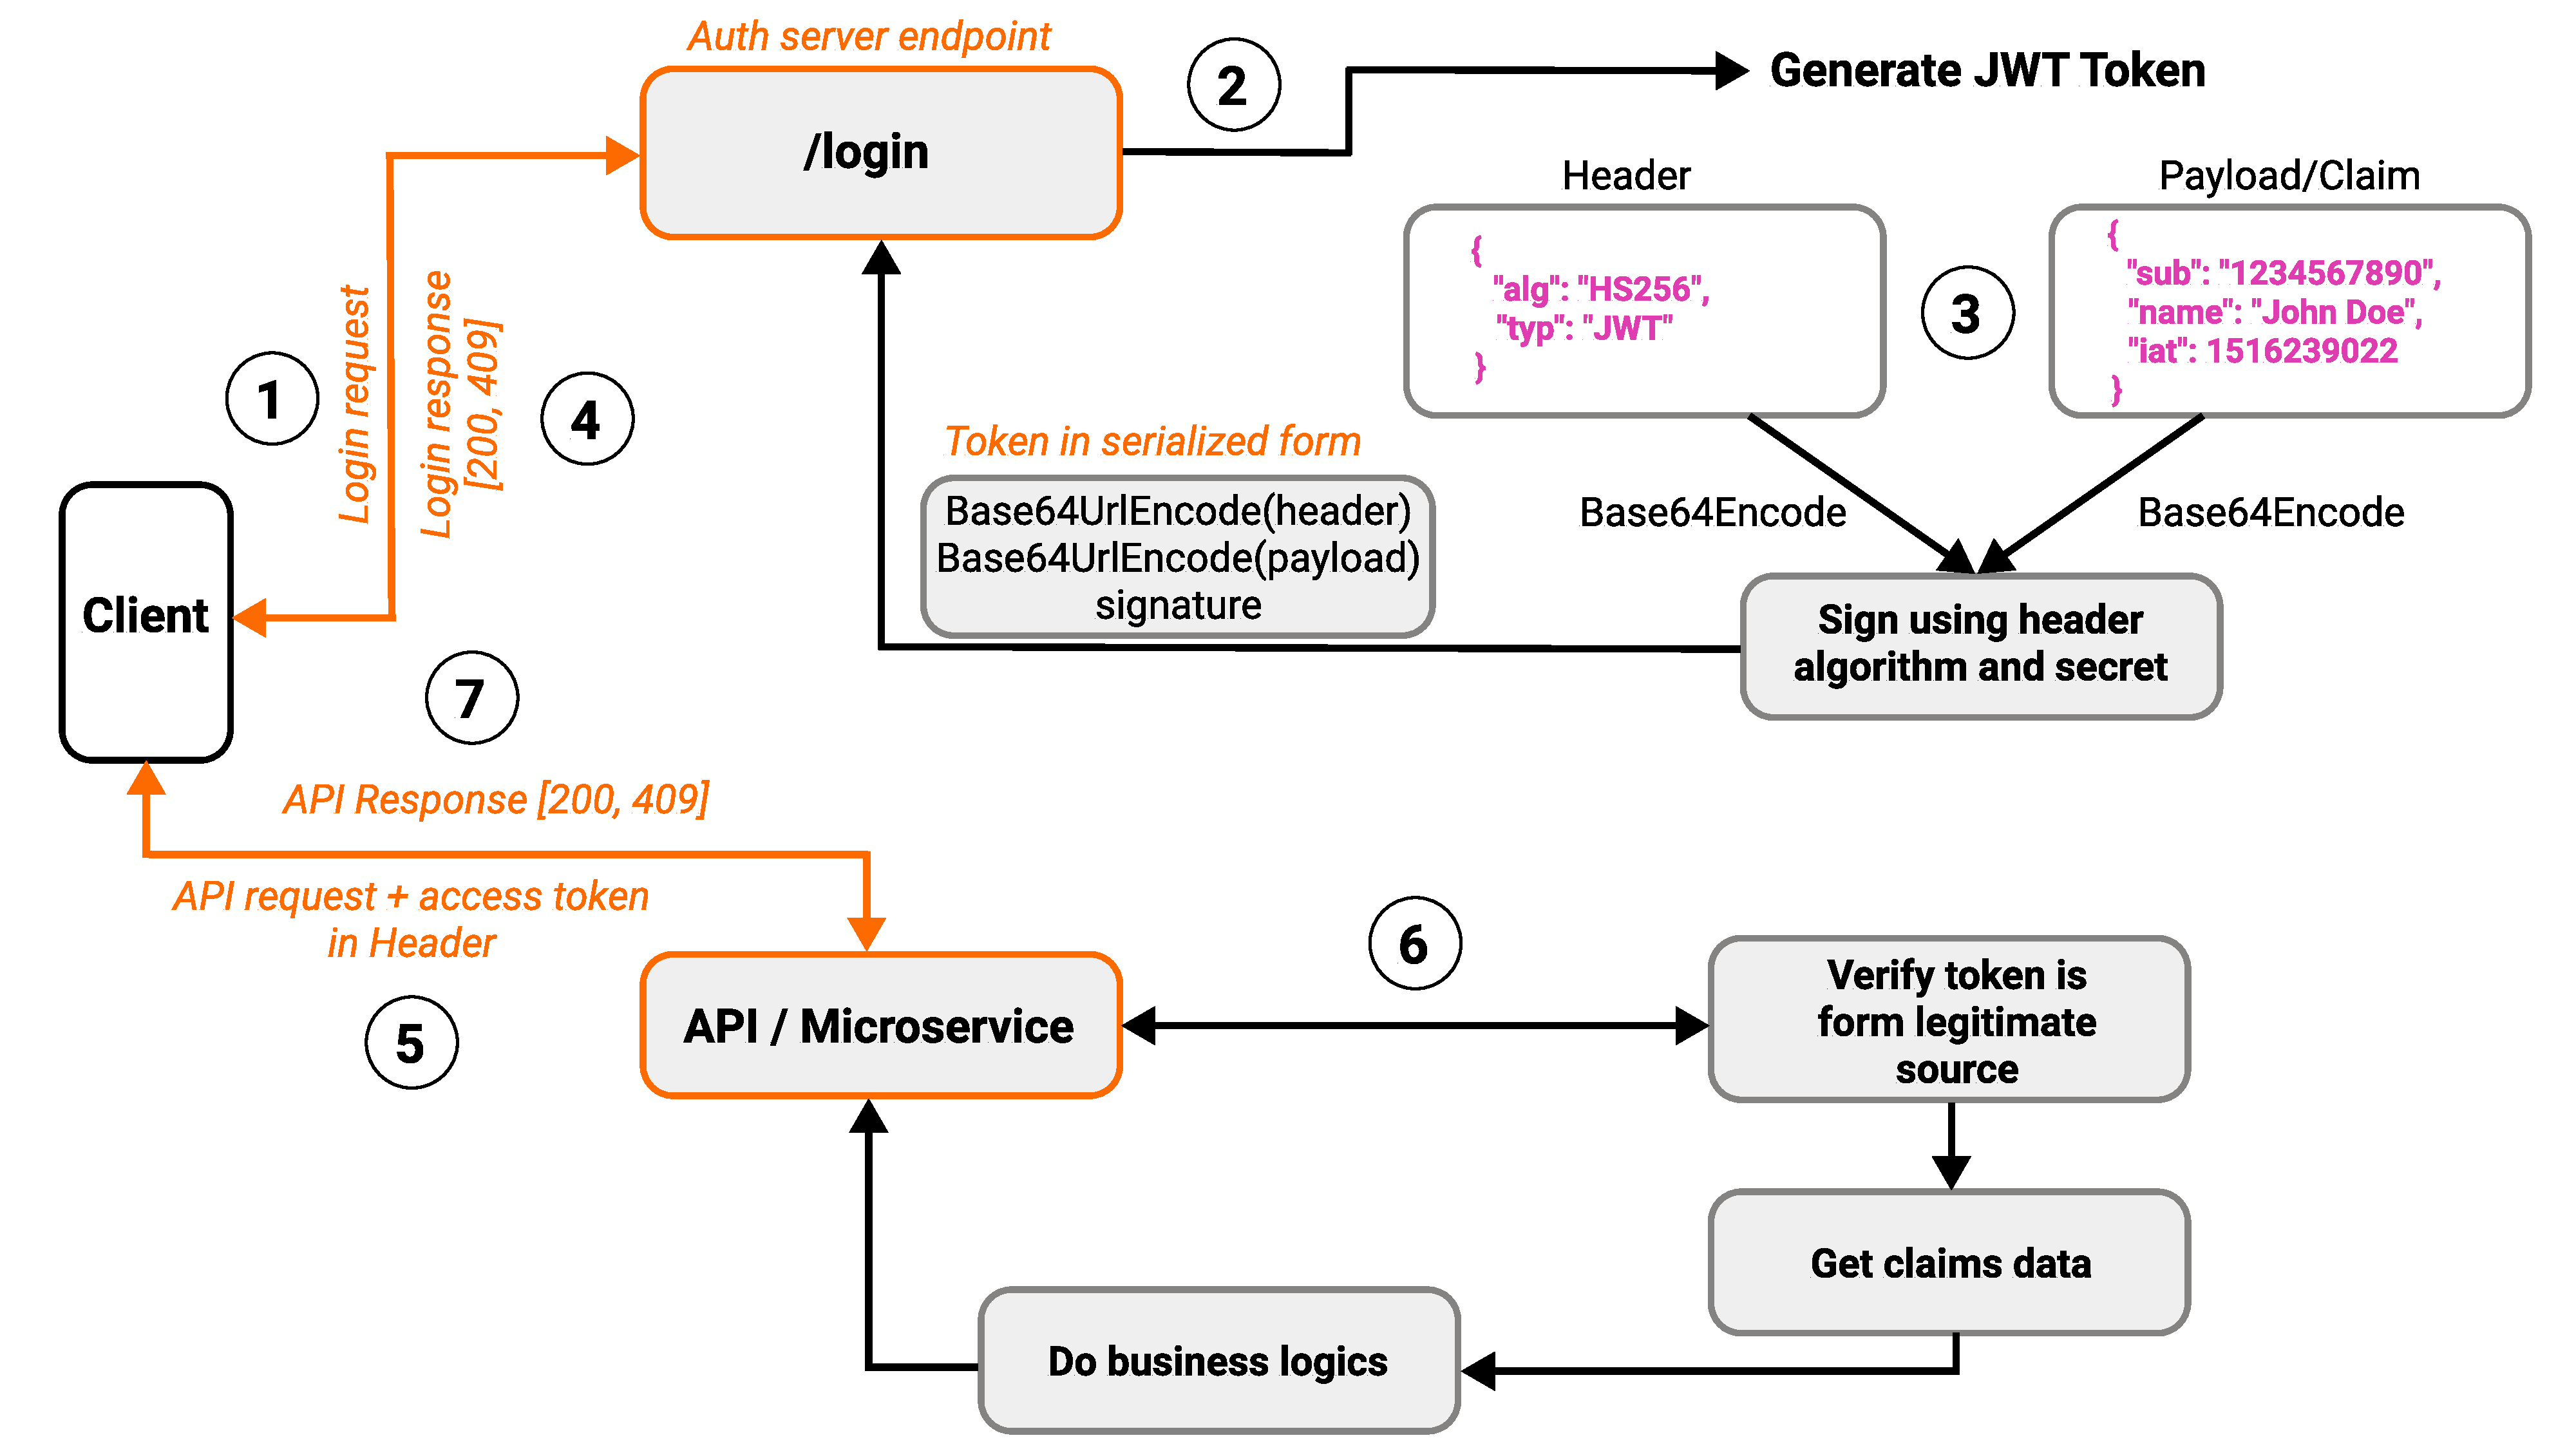
\includegraphics[width=1\textwidth]{Pictures/jwt_auth_scheme.pdf}
    \caption{JWT Authentication principle diagram.}\label{fig:figure3}
\end{figure}

Also, it is worth to add a few basic rules about JWT usage [\cite{RDegges}]
\begin{itemize}
    \item JWT should have a short lifetime, since it cannot be revoked.
    \item JWT should be used in a single time, e.g JWT per request.
\end{itemize}